\section{Preliminary Cuts}

To identify possible candidates several cuts are applied.  

\begin{itemize}
\item{An electron must be detected in the event.}
\item{The difference between the candidate vertex and the electron vertex must be less than 4 cm.  This removes many low momentum tracks that don't come directly from the interaction in the target.}
\item{For positive tracks, a fiducial cut is placed on the drift chamber region 1.}
\end{itemize}

\begin{figure}
  \label{fig:kp_bvp}
  \begin{centering}
    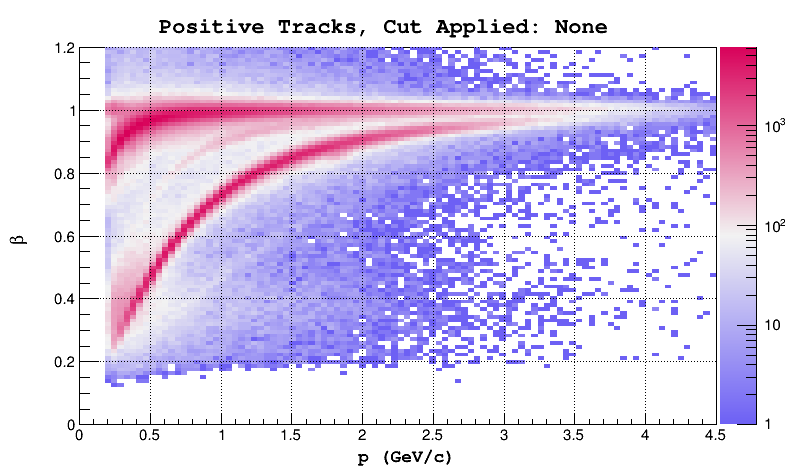
\includegraphics[width=10cm]{image/kp/BetaPNoCutsSector1.png}
    \caption{$\beta (p)$ for positive tracks in sector 1. }
  \end{centering}
\end{figure}

\begin{figure}
  \begin{centering}
    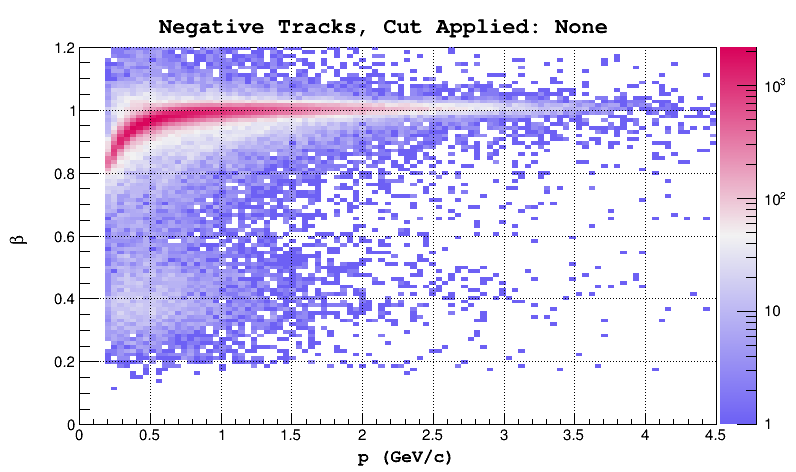
\includegraphics[width=10cm]{image/km/BetaPNoCutsSector1.png}
    \caption{$\beta (p)$ for negative tracks in sector 1. }
  \end{centering}
  \end{figure}

\begin{figure}
  \begin{center}
    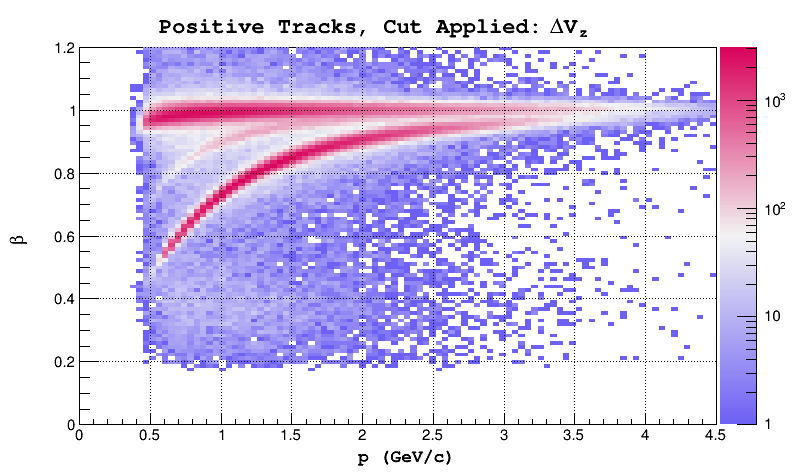
\includegraphics[width=10cm]{image/kp/BetaPDVzCutSector1.png}
    \caption{ $\beta (p)$ for positive tracks passing the $\Delta V_{z}$ cut shown. }
  \end{center}
\end{figure}

\begin{figure}
  \begin{center}
    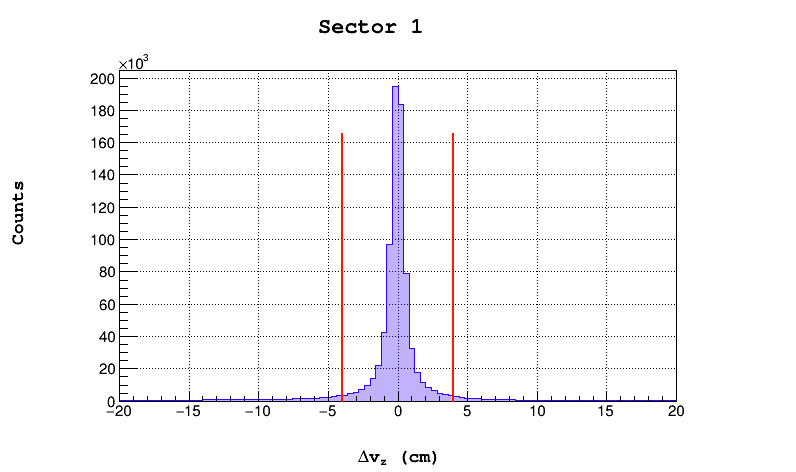
\includegraphics[width=10cm]{image/kp/kp_dvz_sector1.png}
    \caption{The distribution of $\Delta V_{z}$ for positive tracks.}
  \end{center}
\end{figure}

\begin{figure}
  \begin{center}
    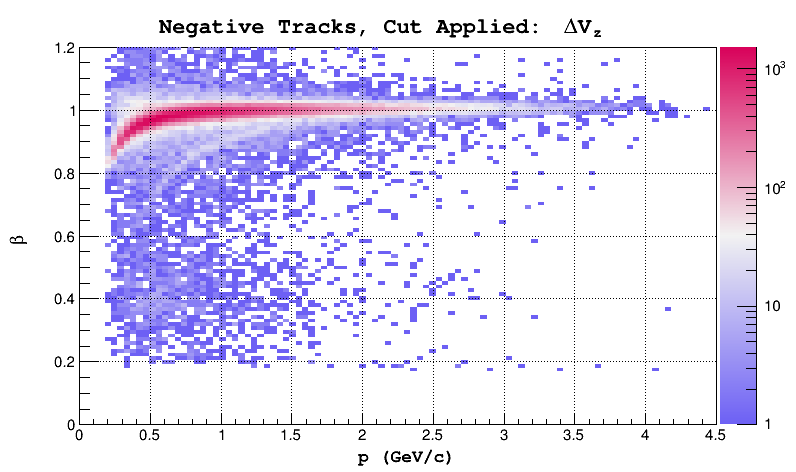
\includegraphics[width=10cm]{image/km/BetaPDVzCutSector1.png}
    \caption{ $\beta (p)$ for negative tracks passing the $\Delta V_{z}$ cut shown. }
  \end{center}
\end{figure}

\begin{figure}
  \begin{center}
    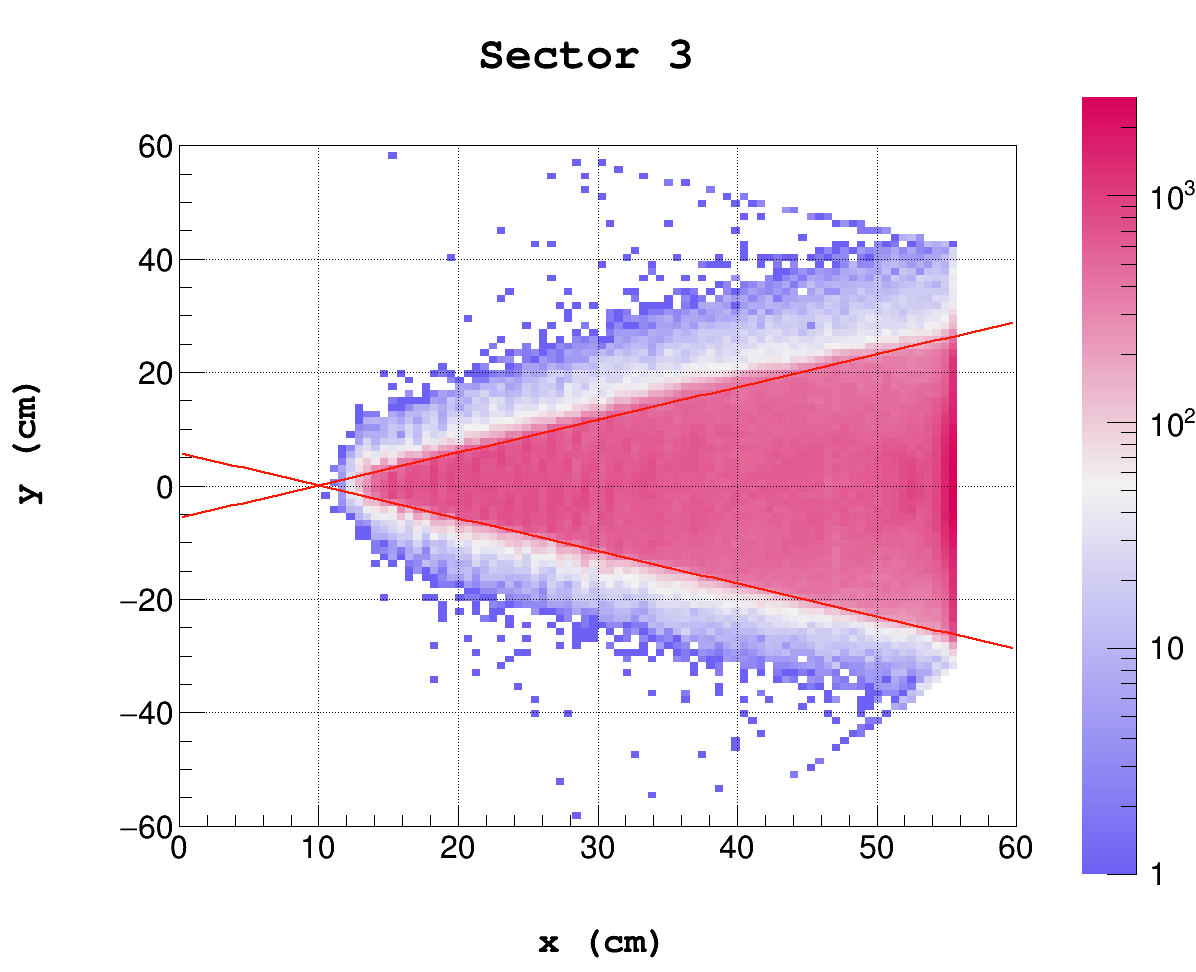
\includegraphics[width=10cm]{image/kp/DCR1Sector3.png}
    \caption{ Positive tracks at the region 1 drift chambers. The red lines illustrate the cut boundary for good tracks (inside).  }
  \end{center}
\end{figure}

The fiducial cut on positive (which bend toward the beamline in the magnetic field used for this experiment) tracks prevents events near the boundaries of the detector (poorly understood effects) from entering our sample.  The cut boundaries intersect 10 cm radially away from the beamline, and open at 60 degrees. 

